
\section{Voice Recognition}

\subsection{Algorithm Used}
\begin{enumerate}
  \item An utterance of a user is collected during the enrollment procedure.
  \item Voice Activity Detection is performed: The silent part of the speech signals must be filtered out to decrease the bias that might occur during training.
  \item Feature Extraction
    \begin{itemize}
      \item Mel-Frequency Cepstral Coefficient (MFCC) is a representation of the short term power spectrum of a sound, based on a linear cosine transform of a log power spectrum on a non-linear mel-scale of frequency. This can be applied to speaker recognition task. The process to extract MFCC feature is demonstrated in Figure \ref{fig:MFCC_fig_one}. \\
      \begin{figure}[!t]
      \centering
      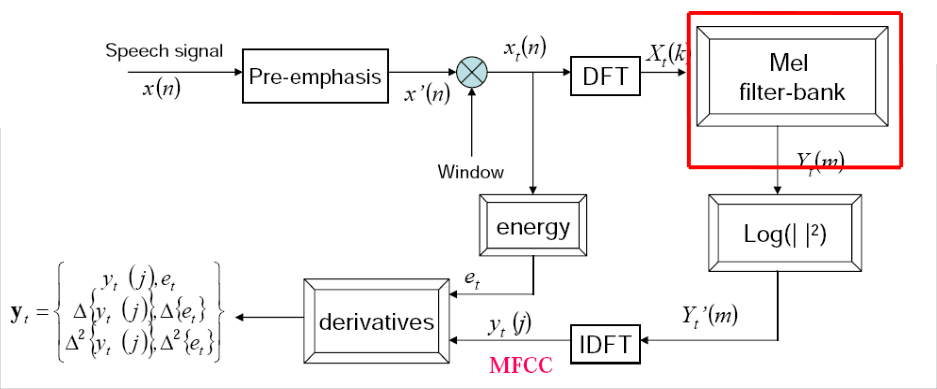
\includegraphics[width=2.5in]{./MFCC-mel-filterbank.png}
      % where an .eps filename suffix will be assumed under latex,
      % and a .pdf suffix will be assumed for pdflatex; or what has been declared
      % via \DeclareGraphicsExtensions.
      \caption{MFCC Feature Extraction Process}
      \label{fig:MFCC_fig_one}
      \end{figure}
      \\
      \item Linear Predictive Coding (LPC) is a tool used in audio signal processing and speech processing for representing the spectral envelope of a digital signal of speech in compressed form, using the information of a Linear predictive Model. \\
      The basic  assumption that is used in LPC is that, the n th signal is a linear combination of the previous p signals. An optimization can be done by the Levinson-Durbin algorithm, to estimate the coefficients ai in the signal, the squared error should be minimized.
    \end{itemize}
    
    \item Gaussian Mixture Model (GMM) is a weighted combination of multivariate Gaussian distribution which assumes feature vectors are independent. This is used in acoustic training task , such as speaker recognition, as it can describe the distribution of all feature vectors. Since the dimensions of the feature vector are independent of each other, diagonal covariance is used.  GMM can also describe the distribution of feature vectors as shown in Figure \ref{fig:GMM_fig_one}. \\

  \begin{figure}[!t]
  \centering
  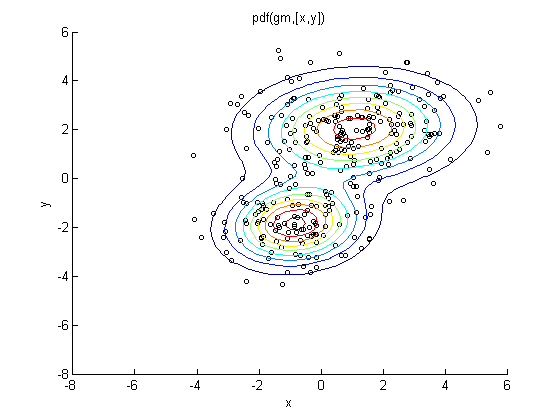
\includegraphics[width=2.5in]{./gmm.png}
  % where an .eps filename suffix will be assumed under latex,
  % and a .pdf suffix will be assumed for pdflatex; or what has been declared
  % via \DeclareGraphicsExtensions.
  \caption{A Two Dimensional GMM with Two Components}
  \label{fig:GMM_fig_one}
  \end{figure}

  Also, an enhancement has been done to the original GMM method. The training phase requires an initialization of the means of all the components in the GMM. But, we first use K-means algorithm to perform a clustering of all the feature vectors, and then use these clustered centers to initialize the training of the GMM. It has been found that, this can speedup the training and also give a better training result.
  \item Joint Factor Analysis (JFA) is a typical method which behave very well in classification problems, due to its ability to account for different types of variability in training data. Within all the factor analysis methods, JFA was proved to outperform other methods in the task of speaker recognition. \\  JFA models the user by supervector, i.e., a C x F dimension vector, where C is the number of components in the Universal Background Model, trained by GMM on all the training data, and F is the dimension of the acoustic feature vector. The supervector of an utterance is obtained by concatenating all the C means vectors in the trained GMM model.
\end{enumerate}
